\newcommand{\nom}{Porte conteneur}
\newcommand{\sequence}{03}
\newcommand{\num}{04}
\newcommand{\type}{TD}
\newcommand{\descrip}{Résolution d'un problème en utilisant des méthodes algorithmiques}
\newcommand{\competences}{Alt-C3: Concevoir un algorithme répondant à un problème précisément posé}

\documentclass[10pt,a4paper]{article}
  \usepackage[french]{babel}
  \usepackage[utf8]{inputenc}
  \usepackage[T1]{fontenc}
  \usepackage{xcolor}
  \usepackage[]{graphicx}
  \usepackage{makeidx}
  \usepackage{textcomp}
  \usepackage{amsmath}
  \usepackage{amssymb}
  \usepackage{stmaryrd}
  \usepackage{fancyhdr}
  \usepackage{lettrine}
  \usepackage{calc}
  \usepackage{boxedminipage}
  \usepackage[french,onelanguage, boxruled,linesnumbered]{algorithm2e}
  \usepackage[colorlinks=false,pdftex]{hyperref}
  \usepackage{minted}
  \usepackage{url}
  %\usepackage[locale=FR]{siunitx}
  \usepackage{multicol}
  \makeindex

  %\graphicspath{{../Images/}}

  \renewcommand\listingscaption{Programme}

  %\renewcommand{\thechapter}{\Alph{chapter}}
  \renewcommand{\thesection}{\Roman{section}}
  %\newcommand{\inter}{\vspace{0.5cm}%
  %\noindent }
  %\newcommand{\unite}{\ \textrm}
  \newcommand{\ud}{\mathrm{d}}
  \newcommand{\vect}{\overrightarrow}
  %\newcommand{\ch}{\mathrm{ch}} % cosinus hyperbolique
  %\newcommand{\sh}{\mathrm{sh}} % sinus hyperbolique

  \textwidth 160mm
  \textheight 250mm
  \hoffset=-1.70cm
  \voffset=-1.5cm
  \parindent=0cm

  \pagestyle{fancy}
  \fancyhead[L]{\bfseries {\large PTSI -- Dorian}}
  \fancyhead[C]{\bfseries{{\type} \no \num}}
  \fancyhead[R]{\bfseries{\large Informatique}}
  \fancyfoot[C]{\thepage}
  \fancyfoot[L]{\footnotesize R. Costadoat, J. Genzmer, W. Robert}
  \fancyfoot[R]{\small \today}
  
  \definecolor{bg}{rgb}{0.5,0.5,0.5}
  \definecolor{danger}{RGB}{217,83,79}
  
  \fancypagestyle{correction}{%
  \fancyhf{}
  \lhead{\colorbox{danger}{\begin{minipage}{0.65\paperwidth} \textcolor{white}{\textbf{Correction}} \end{minipage}} }
  \rhead{
\includegraphics[width=2cm]{../../img/logo}}
  \lfoot{Juliette Genzmer, Willie Robert, Renaud Costadoat}
  \rfoot{\colorbox{danger}{\begin{minipage}{0.6\paperwidth} \begin{flushright}\textcolor{white}{\textbf{Correction}}\end{flushright} \end{minipage}} }}

  
  % macro Juliette
  
\usepackage{comment}   
\usepackage{amsthm}  
\theoremstyle{definition}
\newtheorem{exercice}{Exercice}
\newtheorem*{rappel}{Rappel}
\newtheorem*{remark}{Remarque}
\newtheorem*{defn}{Définition}
\newtheorem*{ppe}{Propriété}
\newtheorem{solution}{Solution}


\begin{document}

\section{Présentation du système}

\begin{minipage}{0.45\linewidth}
La barrière Sympact s'ouvre grâce à l'action d'un moteur et d'un ressort. Utilisée sur un péage et lorsque le moteur n'est pas alimenté (coupure de courant), la barrière doit s'ouvrir afin de permettre aux utilisateurs de passer.
\end{minipage}\hfill
\begin{minipage}{0.45\linewidth}
\begin{center}
 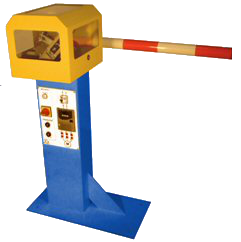
\includegraphics[width=0.8\linewidth]{img/sympact.png}
\end{center}
\end{minipage}

~\

La barrière installée en salle de TP ne pouvant pas mesure 2.5m, des masses équivalentes ont été ajoutées. La masse de la lisse sera donc assimilée à ces masses:
\begin{itemize}
 \item une masse $m_1=2.8kg$ située à $l_1=170mm$ de son axe de rotation,
 \item une masse $m_2=1kg$ située à $l_2=1170mm$ de son axe de rotation.
\end{itemize}

Son inertie ramenée sur l'arbre sera donc: $J_{eq}=m_1*l_1^2+m_2*l_2^2$.

\section{Étude de la dynamique de la barrière}

\paragraph{Question 1:} Réaliser un schéma cinématique paramétré de la barrière.

\paragraph{Question 2:} Déterminer l'action mécanique du poids de la lisse ramenée sur l'axe de rotation de la lisse.

Lors de la phase d'ouverture non-alimentée, la lisse est soumise:
\begin{itemize}
 \item A son poids,
 \item A l'action du ressort de raideur $K=0.45N.m/deg$ et de position à l'équilibre $\theta_0=90°$,
 \item Des frottements visqueux de coefficient $\lambda=4N.m.s/rad$.
\end{itemize}

\paragraph{Question 3:} Après avoir isolé la lisse, écrire le Principe Fondamental de la Dynamique appliqué sur l'axe de rotation de la lisse. 

\paragraph{Question 4:} Déterminer les profils de la position et de la vitesse de rotation de la lisse à chaque instant en utilisant la méthode d'Euler. La barrière sera considéré immobile et horizontale au départ de l'étude.

\paragraph{Question 5:} Déterminer l'influence du coefficient de frottement sur le système. En sachant que ce coefficient n'est pas aussi important dans le système réel, que se passe-t-il si on diminue sa valeur ? Quel composant du système permet de compenser la diminution du coefficient de frottement.
\end{document}
